\documentclass[border=4pt,12pt]{standalone}
% House style for redrawn exam diagrams (diagram-v4: 0.4pt lines, filled -latex arrows, fine dashes; stipple and hatching drawn as real dots/lines (no PDF/SVG patterns, so they render in every browser and at any scale); transparent background). Every figure \input's this.
\usepackage{amsmath,amssymb}
\usepackage{txfonts}
\usepackage{pdfrender,xcolor}
% \halo{text}: label on shading. The shading stops just around each letter's outline (a thin knock-out that follows the
% glyphs, like the papers' typesetting), never a box. Owner: "I don't want a box around the text".
\newcommand{\halo}[1]{\leavevmode\rlap{\pdfrender{TextRenderingMode=2,LineWidth=2.2pt,LineJoinStyle=1,StrokeColor=white,FillColor=white}#1}#1}
\usepackage{tikz,pgfplots}
\pgfplotsset{compat=1.18}
\usetikzlibrary{arrows.meta,calc,angles,quotes,patterns,patterns.meta,intersections,positioning,decorations.markings,shapes.geometric}
% Stipple and hatching are drawn as actual dots / lines clipped to the region (path picture), NOT as pattern fills:
% SVG <pattern> fills vanish or blur when browsers scale the image, so the owner could not see the shading.
% Each dot is a 0.72pt square (keeps SVGs small; reads as a dot at print size). Dots sit on one global staggered grid, so neighbouring regions line up.
\makeatletter
\newdimen\ex@x \newdimen\ex@y \newdimen\ex@xa \newdimen\ex@ya \newdimen\ex@xb \newdimen\ex@yb \newcount\ex@row
\def\exam@stipplecolor{black!75}\def\exam@dotr{0.42pt}\def\exam@dotgap{2.5}
\def\ex@rowdots{\ifdim\ex@x<\ex@xb \pgfpathrectangle{\pgfqpoint{\dimexpr\ex@x-0.36pt\relax}{\dimexpr\ex@y-0.36pt\relax}}{\pgfqpoint{0.72pt}{0.72pt}}\advance\ex@x by \exam@dotgap pt\relax\expandafter\ex@rowdots\fi}
\def\exam@stipple{%
  \pgftransformreset% dots are sized in real points even inside scaled pictures
  \pgfpointanchor{path picture bounding box}{south west}\ex@xa=\pgf@x \ex@ya=\pgf@y
  \pgfpointanchor{path picture bounding box}{north east}\ex@xb=\pgf@x \ex@yb=\pgf@y
  \pgfsetfillcolor{\exam@stipplecolor}\pgfmathsetmacro\ex@h{\exam@dotgap/2}%
  \pgfmathtruncatemacro\ex@r{floor(\ex@ya/\ex@h)-1}\ex@row=\ex@r\relax
  \ex@y=\ex@r\dimexpr\ex@h pt\relax
  \loop\ifdim\ex@y<\ex@yb
    \pgfmathtruncatemacro\ex@c{floor(\ex@xa/\exam@dotgap)-1}\ex@x=\ex@c\dimexpr\exam@dotgap pt\relax
    \ifodd\ex@row \advance\ex@x by \ex@h pt\fi
    \ex@rowdots
    \advance\ex@y by \ex@h pt \advance\ex@row by 1
    \ifnum\numexpr\ex@row-(\ex@row/4)*4\relax=0 \pgfusepath{fill}\fi% flush every 4 rows: bounded TeX memory, few clip copies in the SVG
  \repeat\pgfusepath{fill}}
\newdimen\ex@d
\def\exam@hatch#1{% #1 = 1 for /, -1 for \ ; lines 45 degrees, 3pt apart
  \pgftransformreset
  \pgfpointanchor{path picture bounding box}{south west}\ex@xa=\pgf@x \ex@ya=\pgf@y
  \pgfpointanchor{path picture bounding box}{north east}\ex@xb=\pgf@x \ex@yb=\pgf@y
  \ex@d=\dimexpr\ex@yb-\ex@ya\relax \ex@x=\dimexpr\ex@xa-\ex@d\relax
  \loop\ifdim\ex@x<\ex@xb
    \ifnum#1>0 \pgfpathmoveto{\pgfqpoint{\ex@x}{\ex@ya}}\pgfpathlineto{\pgfqpoint{\dimexpr\ex@x+\ex@d\relax}{\ex@yb}}%
    \else \pgfpathmoveto{\pgfqpoint{\ex@x}{\ex@yb}}\pgfpathlineto{\pgfqpoint{\dimexpr\ex@x+\ex@d\relax}{\ex@ya}}\fi
    \advance\ex@x by 4.24pt
  \repeat
  \pgfsetlinewidth{0.4pt}\pgfsetstrokecolor{black}\pgfusepath{stroke}}
\def\examstipple{\exam@stipple}\def\examhatch{\exam@hatch}\def\examsetstipplecolor#1{\def\exam@stipplecolor{#1}}\def\examsetdotgap#1{\def\exam@dotgap{#1}}
\makeatother
% (legacy pattern kept for old files)
% staggered stipple like the NESA papers' dotted shading
\pgfdeclarepatternformonly{exam stipple}{\pgfpointorigin}{\pgfqpoint{2.2pt}{2.2pt}}{\pgfqpoint{2.2pt}{2.2pt}}{%
  \pgfpathcircle{\pgfqpoint{0.55pt}{0.55pt}}{0.42pt}\pgfpathcircle{\pgfqpoint{1.65pt}{1.65pt}}{0.42pt}\pgfusepath{fill}}
\tikzset{
  every picture/.style={line width=0.6pt, >={Latex[length=2mm,width=1.3mm]}},
  curve/.style={line width=0.6pt},
  open arrow/.style={-{Latex[length=2mm,width=1.3mm]}},  % owner: filled -latex heads everywhere, no open chevrons
  aux/.style={dash pattern=on 2pt off 1.5pt, line width=0.6pt},
  shade/.code={\def\exA{#1}\def\exB{none}\ifx\exA\exB\else\pgfkeysalso{fill=black!18}\fi},
  shade/.default=on,
  shade dots/.style={fill=none, path picture={\examstipple}},
  stipple color/.code={\examsetstipplecolor{#1}},
  stipple gap/.code={\examsetdotgap{#1}},
  shade dense dots/.style={fill=none, stipple gap=1.6, path picture={\examstipple}},
  shade hatch/.style={fill=none, path picture={\examhatch{1}}},
  shade hatch reverse/.style={fill=none, path picture={\examhatch{-1}}},
  shade solid/.style={fill=black},
  pt/.style={circle, fill, inner sep=1.1pt},
  open pt/.style={circle, draw, fill=white, inner sep=1.1pt},
}
\pgfplotsset{
  exam axes/.style={axis lines=middle, axis line style={->}, xlabel={$x$}, ylabel={$y$},
    xlabel style={anchor=west}, ylabel style={anchor=south}, tick label style={font=\small},
    every axis plot/.append style={line width=0.6pt, black}, samples=200, clip=false,
    enlargelimits=false, axis on top},
}

\begin{document}
% 638_q6_s1: the school's solution overlays -f(x), -f(-x) and -f(2-x) in three colours on one set of axes. Black and white
% only (rule 6), so the three stages are drawn as three panels in a row, each from the f traced for 638_q6_1 and transformed
% exactly: -f(x) reflects in the x-axis (asymptote x=2), -f(-x) then in the y-axis (x=-2), -f(2-x) shifts 2 right (x=0),
% which is the g(x) of the question. Panel units = 638_q6_1 crop pixels relative to its origin, scaled 0.6. The handwritten
% notes are left out: they are the solution text.
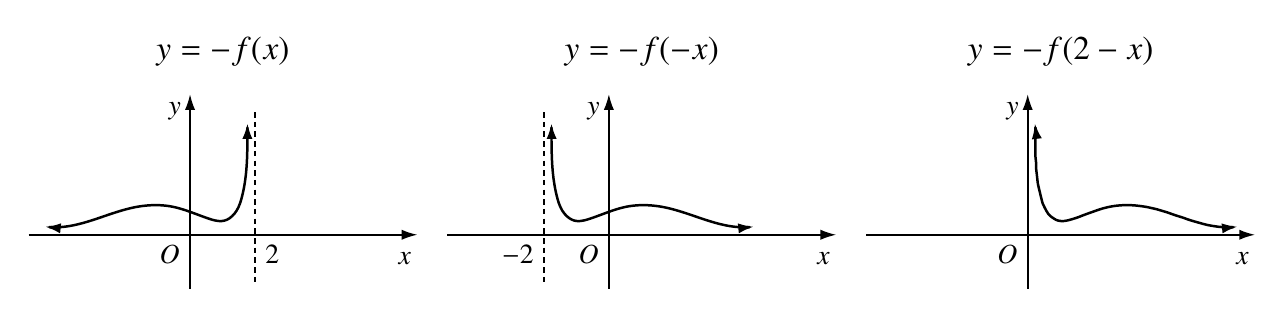
\begin{tikzpicture}[x=0.0076cm, y=-0.0076cm]
  % panel 1: y = -f(x)
  \draw[->] (-270,0) -- (380,0) node[below left, inner sep=2pt, yshift=-4pt] {$x$};
  \draw[->] (0,90) -- (0,-235) node[left, inner sep=3pt, yshift=-6pt] {$y$};
  \draw[aux] (108.5,-205) -- (108.5,85);
  \draw[<->, line width=0.9pt] plot[smooth] coordinates {(-242.5,-13.5) (-234.5,-12.74) (-226.6,-12.47) (-218.6,-12.68) (-210.4,-13.36) (-202.2,-14.48) (-194,-16.01) (-185.6,-17.93) (-177.1,-20.18) (-168.6,-22.71) (-159.8,-25.5) (-151,-28.46) (-142,-31.56) (-133,-34.6) (-124.2,-37.47) (-115.5,-40.15) (-107,-42.55) (-98.69,-44.63) (-90.26,-46.39) (-81.98,-47.76) (-73.65,-48.75) (-65.29,-49.35) (-57.05,-49.54) (-48.84,-49.3) (-40.8,-48.63) (-32.84,-47.51) (-24.98,-45.93) (-16.98,-43.85) (-8.708,-41.32) (-0.3529,-38.45) (8.349,-35.27) (17.33,-31.93) (25.93,-28.8) (34.18,-25.99) (41.27,-24.02) (47.37,-23.01) (52.66,-22.89) (57.37,-23.6) (61.6,-25.1) (65.94,-27.58) (70.26,-31.05) (74.38,-35.46) (77.85,-40.35) (80.94,-46.1) (83.51,-52.47) (85.83,-59.97) (87.9,-68.15) (89.71,-76.59) (91.24,-85.18) (92.5,-93.91) (93.53,-102.8) (94.32,-111.7) (94.91,-120.7) (95.34,-129.9) (95.61,-139) (95.78,-148.3) (95.87,-157.8) (95.91,-167.4) (95.94,-176.9) (96,-186.5)};
  \node[anchor=north east, inner sep=3pt] at (-2,2) {$O$};
  \node[anchor=north west, inner sep=3pt] at (110.5,2) {$2$};
  \node[anchor=south, font=\large] at (55,-265) {$y=-f(x)$};
  % panel 2: y = -f(-x)
  \draw[->] (430,0) -- (1080,0) node[below left, inner sep=2pt, yshift=-4pt] {$x$};
  \draw[->] (700,90) -- (700,-235) node[left, inner sep=3pt, yshift=-6pt] {$y$};
  \draw[aux] (591.5,-205) -- (591.5,85);
  \draw[<->, line width=0.9pt] plot[smooth] coordinates {(942.5,-13.5) (934.5,-12.74) (926.6,-12.47) (918.6,-12.68) (910.4,-13.36) (902.2,-14.48) (894,-16.01) (885.6,-17.93) (877.1,-20.18) (868.6,-22.71) (859.8,-25.5) (851,-28.46) (842,-31.56) (833,-34.6) (824.2,-37.47) (815.5,-40.15) (807,-42.55) (798.7,-44.63) (790.3,-46.39) (782,-47.76) (773.7,-48.75) (765.3,-49.35) (757.1,-49.54) (748.8,-49.3) (740.8,-48.63) (732.8,-47.51) (725,-45.93) (717,-43.85) (708.7,-41.32) (700.4,-38.45) (691.7,-35.27) (682.7,-31.93) (674.1,-28.8) (665.8,-25.99) (658.7,-24.02) (652.6,-23.01) (647.3,-22.89) (642.6,-23.6) (638.4,-25.1) (634.1,-27.58) (629.7,-31.05) (625.6,-35.46) (622.1,-40.35) (619.1,-46.1) (616.5,-52.47) (614.2,-59.97) (612.1,-68.15) (610.3,-76.59) (608.8,-85.18) (607.5,-93.91) (606.5,-102.8) (605.7,-111.7) (605.1,-120.7) (604.7,-129.9) (604.4,-139) (604.2,-148.3) (604.1,-157.8) (604.1,-167.4) (604.1,-176.9) (604,-186.5)};
  \node[anchor=north east, inner sep=3pt] at (698,2) {$O$};
  \node[anchor=north east, inner sep=3pt] at (589.5,2) {$-2$};
  \node[anchor=south, font=\large] at (755,-265) {$y=-f(-x)$};
  % panel 3: y = -f(2-x)
  \draw[->] (1130,0) -- (1780,0) node[below left, inner sep=2pt, yshift=-4pt] {$x$};
  \draw[->] (1400,90) -- (1400,-235) node[left, inner sep=3pt, yshift=-6pt] {$y$};
  \draw[<->, line width=0.9pt] plot[smooth] coordinates {(1751,-13.5) (1743,-12.74) (1735,-12.47) (1727,-12.68) (1719,-13.36) (1711,-14.48) (1702,-16.01) (1694,-17.93) (1686,-20.18) (1677,-22.71) (1668,-25.5) (1660,-28.46) (1650,-31.56) (1641,-34.6) (1633,-37.47) (1624,-40.15) (1616,-42.55) (1607,-44.63) (1599,-46.39) (1590,-47.76) (1582,-48.75) (1574,-49.35) (1566,-49.54) (1557,-49.3) (1549,-48.63) (1541,-47.51) (1533,-45.93) (1525,-43.85) (1517,-41.32) (1509,-38.45) (1500,-35.27) (1491,-31.93) (1483,-28.8) (1474,-25.99) (1467,-24.02) (1461,-23.01) (1456,-22.89) (1451,-23.6) (1447,-25.1) (1443,-27.58) (1438,-31.05) (1434,-35.46) (1431,-40.35) (1428,-46.1) (1425,-52.47) (1423,-59.97) (1421,-68.15) (1419,-76.59) (1417,-85.18) (1416,-93.91) (1415,-102.8) (1414,-111.7) (1414,-120.7) (1413,-129.9) (1413,-139) (1413,-148.3) (1413,-157.8) (1413,-167.4) (1413,-176.9) (1412,-186.5)};
  \node[anchor=north east, inner sep=3pt] at (1398,2) {$O$};
  \node[anchor=south, font=\large] at (1455,-265) {$y=-f(2-x)$};
\end{tikzpicture}
\end{document}
